%%%%%%%%%%%%%%%%%%%%%%%%%%%%%%%%%%%%%%%%%%%%%%%%%%%%%%%%%%%%%%%%%%%%%%%%%%%%%%%
\chapter{Oscilações}
\label{Chap:ExpOscilacoes}
%%%%%%%%%%%%%%%%%%%%%%%%%%%%%%%%%%%%%%%%%%%%%%%%%%%%%%%%%%%%%%%%%%%%%%%%%%%%%%%

\begin{fullwidth}\it
	Verificaremos o comportamento oscilatório de dois sistemas -- um sistema massa-mola e um pêndulo simples --. Veremos que através das Leis de Newton, chegamos a uma equação cuja solução é uma função periódica que descreve o movimento oscilatório observado. Utilizaremos os seguintes conceitos/técnicas de análise de dados: medidas, algarismos significativos, gráficos, erros de escala e propagados, equação geral para o erro propagado, regressão linear, linearização, e erros dos coeficientes $A$ e $B$.
\end{fullwidth}

%%%%%%%%%%%%%%%%%%%%%%%%%%%%%%%%%%%%%%%%%%%%%%%%%%%%%%%%%%%%%%%%%%%%%%%%%%%%%%%
\section{Sistema massa-mola}
%%%%%%%%%%%%%%%%%%%%%%%%%%%%%%%%%%%%%%%%%%%%%%%%%%%%%%%%%%%%%%%%%%%%%%%%%%%%%%%

Sabemos que a força exercida por uma mola é proporcional à sua distensão:
\begin{align}
	F &= -k\Delta x \\
	&= -kx,
\end{align}
%
onde assumimos que $x_0 = 0$, $k$ é uma constante de proporcionalidade e o sinal negativo significa que a força é no sentido contrário à distensão da mola.

\begin{marginfigure}
	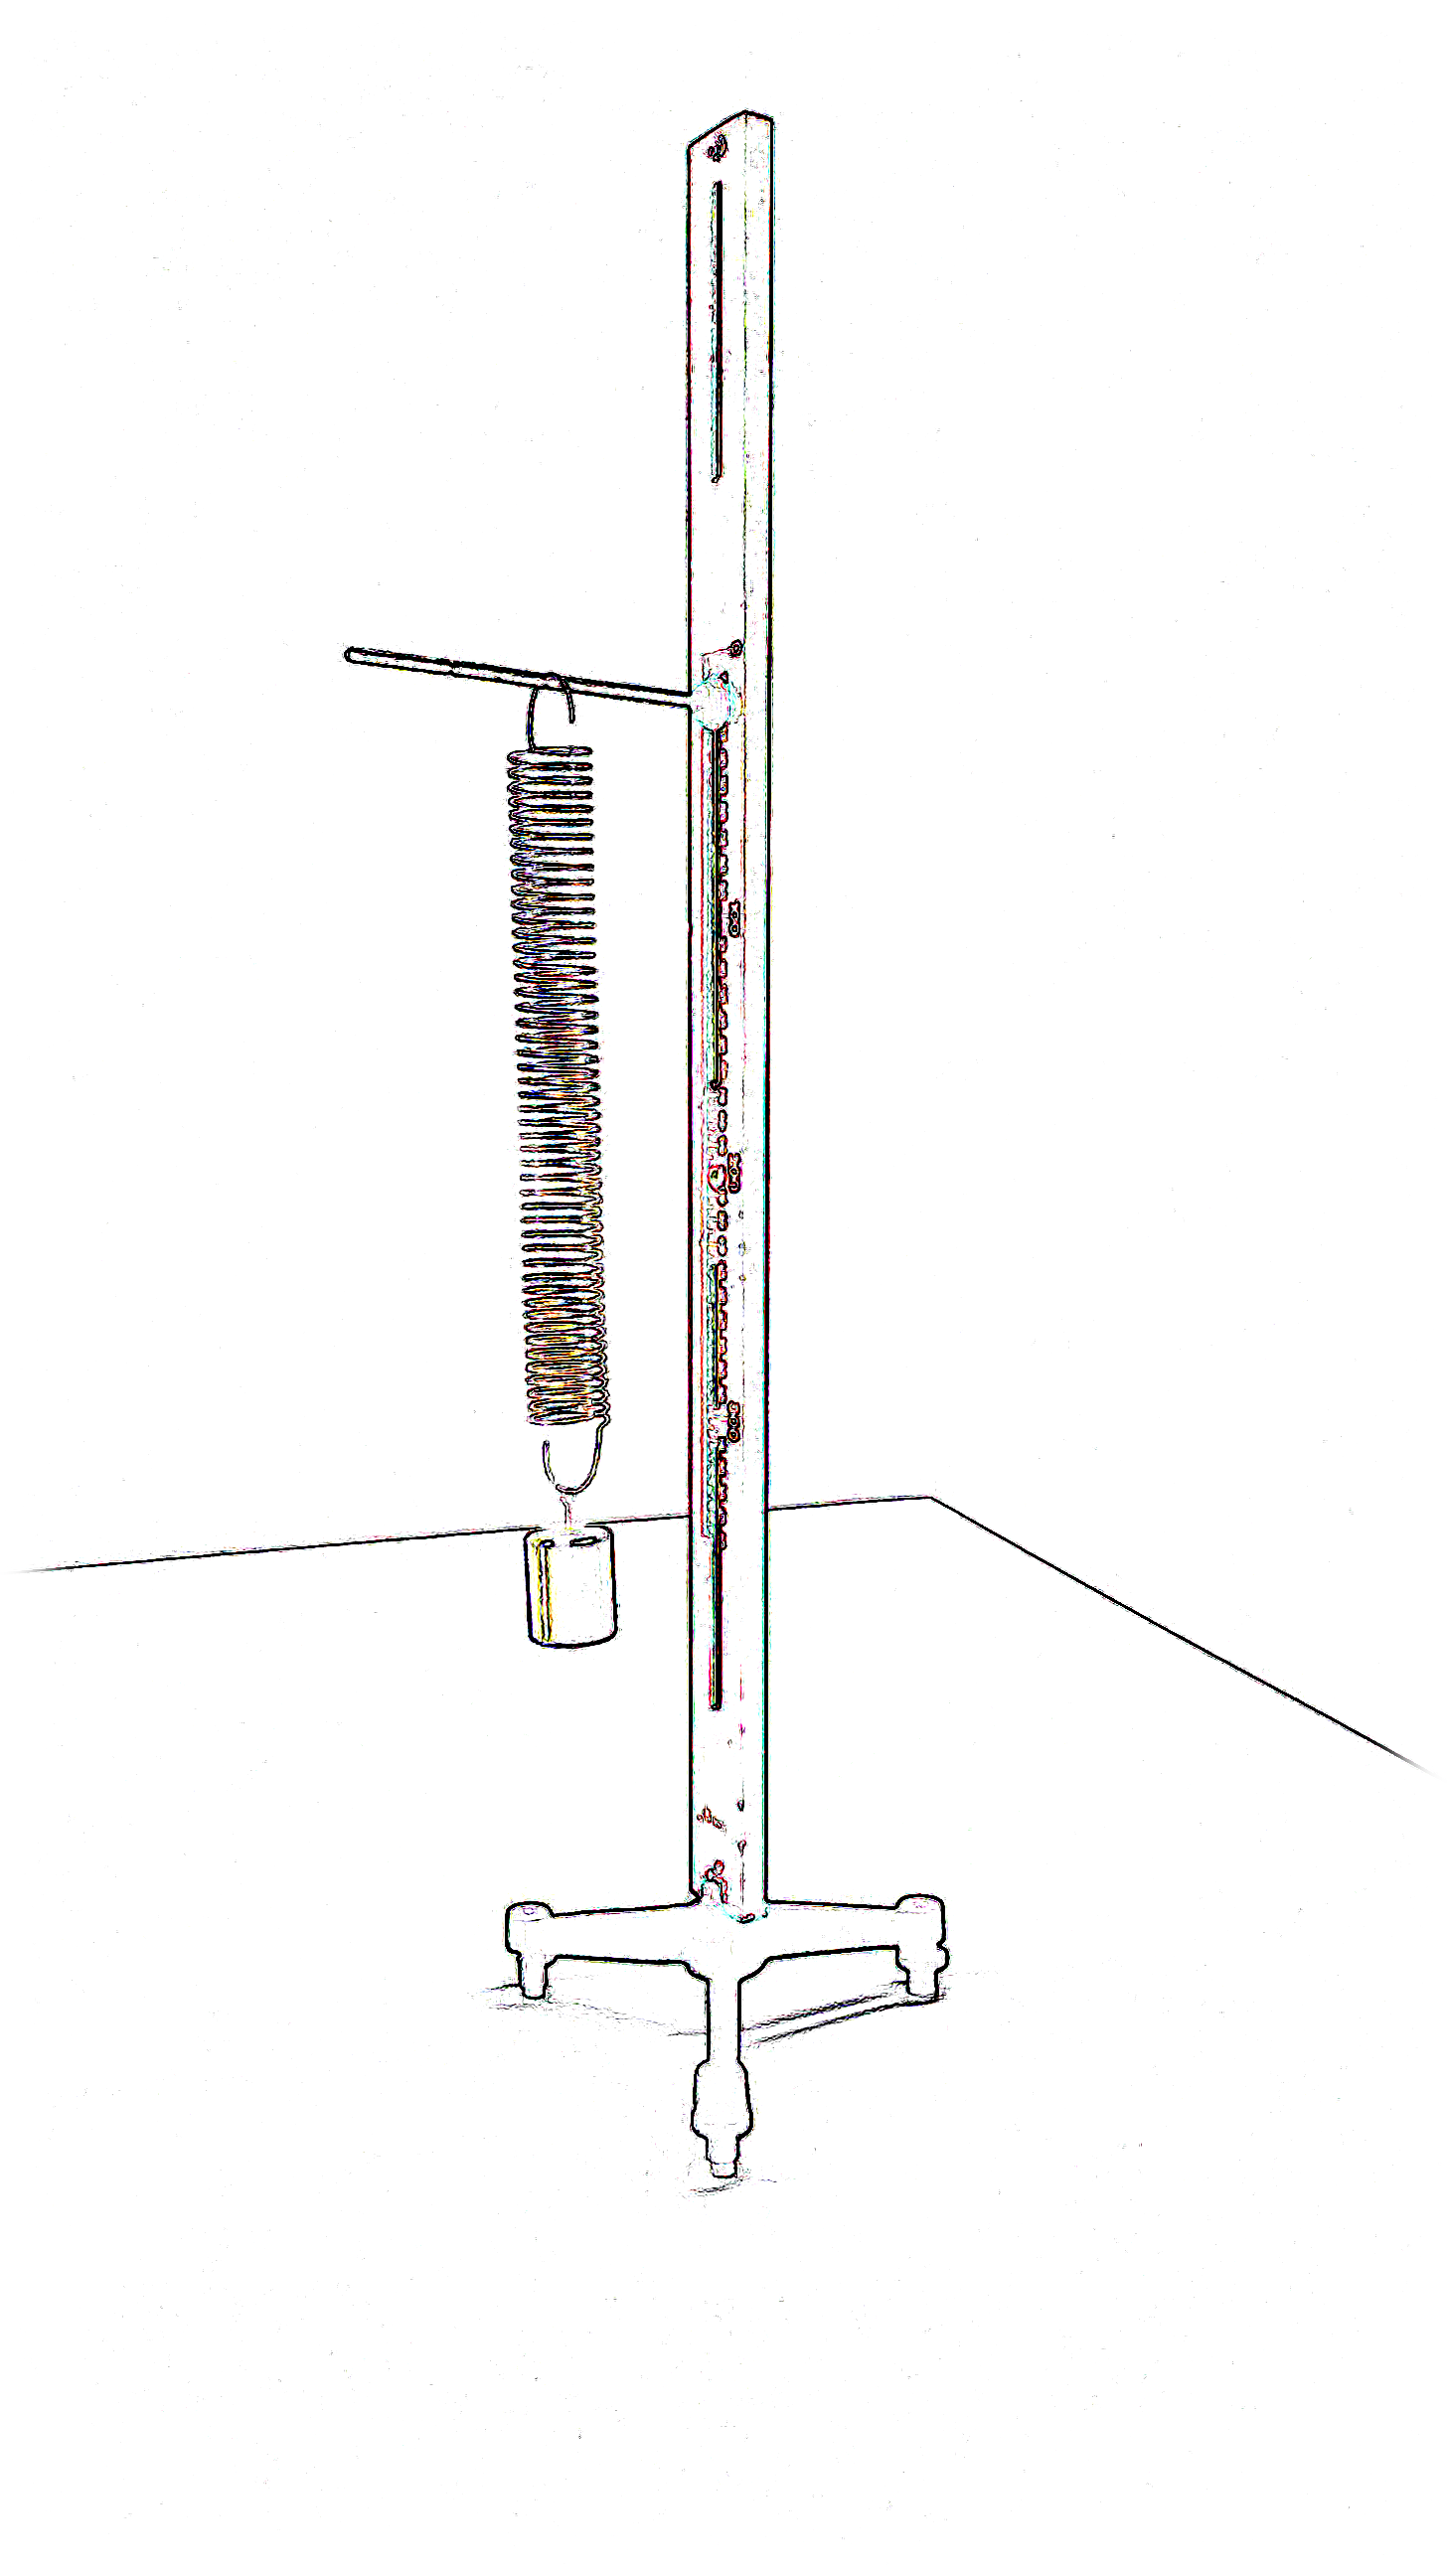
\includegraphics[width=\textwidth]{Ilustrations/Massa-Mola.png}
	\caption{Sistema massa-mola.}
\end{marginfigure}

Se pendurarmos uma mola em um suporte -- de forma que ela se disponha verticalmente -- e prendermos um corpo de massa apreciável à extremidade inferior. Deixamos o corpo descer até que a força exercida pela mola equilibre o peso. A partir dessa posição de equilíbrio, qualquer deslocamento exercido fará com que atue sobre o corpo uma força proporcional ao deslocamento, porém com sentido contrário a ele. Utilizando a segunda lei de Newton, podemos descrever a dinâmica do corpo através de
\begin{equation}
	-kx = ma.
\end{equation}
%
Analisando essa equação, temos que sempre que o corpo se desloca em relação à posição de equilíbrio, ele está sujeito a uma força contraria a esse deslocamento, acelerando-o em direção à posição de deslocamento zero (ou seja, a posição de equilíbrio). Quando o objeto passa pela posição de equilíbrio, sua aceleração é zero, porém sua velocidade não, o que o faz passar de tal posição e continuar o movimento oscilatório. Para tentar descrever esse movimento, podemos substituir a aceleração na equação acima por sua definição em termos da derivada segunda da posição em relação ao tempo:
\begin{equation}
	-kx = m\frac{d^2x}{dt^2},
\end{equation}
%
ou, rearranjando os termos,
\begin{equation}\label{Eq:EquacaoDiferencialOHS}
	\frac{d^2x}{dt^2} + \frac{k}{m} x = 0.
\end{equation}

Através da equação acima, percebemos que a posição $x$ como função do tempo satisfaz uma condição curiosa: a posição vezes uma constante mais sua derivada segunda é zero, ou seja, a função $x(t)$ é tal que sua derivada é igual a ela mesma, vezes uma contante. Existem duas funções que satisfazem essa condição: as funções trigonométricas $\sen$ e $\cos$. Se supusermos que $x(t)$ é então da forma
\begin{equation}
	x(t) = A\sen(\omega t)
\end{equation}
%
e a substituirmos na Equação~\eqref{Eq:EquacaoDiferencialOHS}, temos
\begin{equation}
	-A\omega^2\sen(\omega t) + \frac{k}{m}A\sen(\omega t)=0
\end{equation}
%
o que pode ser simplificado a
\begin{equation}
	\omega^2 = \frac{k}{m}.
\end{equation}

%\begin{marginfigure}
%\centering
%\includegraphics[width=5cm]{Fig/MassaMolaCaneta.png}
%\caption{Sistema massa-mola em que uma caneta foi afixada à massa, riscando sobre uma folha de papel que se move para a esquerda com velocidade constante. Podemos ver que a curva que se forma é uma senoide.}
%\end{marginfigure}

Verificamos então que a forma suposta para $x(t)$ é solução da Equação~\eqref{Eq:EquacaoDiferencialOHS} se $\omega = \sqrt{k/m}$. Portanto, concluímos que a posição do objeto descreve uma curva senoidal em um gráfico da posição em função do tempo. A partir da expressão para a posição, podemos calcular a velocidade e a aceleração em função do tempo
\begin{align}
	v(t) &= A\omega\cos\omega t \\
	a(t) &= -A\omega^2\sen\omega t.
\end{align}

Se analisarmos a função seno, vemos que ela tem um período igual a $2\pi$, isto é, seu gráfico se repete a cada $2\pi$ radianos. Isso se reflete em um ciclo de oscilação do sistema massa mola, pois após o argumento do seno atingir $2\pi$, o movimento se repete. Se considerarmos que o tempo para completar uma oscilação é o período $T$, temos, no instante que o objeto termina uma oscilação
\begin{equation}
	\omega T = 2\pi
\end{equation}
%
o que leva à seguinte equação para o período:
\begin{equation}
	T = 2\pi \frac{1}{\omega}.
\end{equation}
%
Substituindo a expressão para $\omega$, temos
\begin{equation}
	T = 2\pi \sqrt{\frac{m}{k}}.
\end{equation}
%
Verificamos então que o período de oscilação do sistema massa-mola depende da massa do objeto e da constante $k$ da mola.

Expressões como a Equação~\eqref{Eq:EquacaoDiferencialOHS} são comuns em física e são denominadas \emph{Equações Diferenciais Ordinárias}. As soluções para estas equações são \emph{funções}. A Equação~\eqref{Eq:EquacaoDiferencialOHS} em particular define o \emph{Movimento Harmônico Simples}.

%%%%%%%%%%%%%%%%%%%%%%%%%%%%%%%%%%%%%%%%%%%%%%%%%%%%%%%%%%%%%%%%%%%%%%%%%%%%%%%
\section{Pêndulo Simples}
%%%%%%%%%%%%%%%%%%%%%%%%%%%%%%%%%%%%%%%%%%%%%%%%%%%%%%%%%%%%%%%%%%%%%%%%%%%%%%%

Podemos tratar um objeto que oscila preso a uma corda de massa desprezível como uma oscilação harmônica desde que o ângulo máximo de oscilação -- isto é, a amplitude -- seja pequena. Se essa condição for garantida, o pêndulo é denominado \emph{pêndulo simples}.

Se deslocarmos um pêndulo para a direita, como na Figura~\ref{Fig:Pendulo}, teremos uma componente da força peso que tende a restaurar o pêndulo à posição de equilíbrio. Podemos ver que tal componente tem valor $P_t=P\sen\theta$, onde $P=mg$ representa o peso. De acordo com a segunda lei de Newton, temos então
\begin{equation}
	-mg\sen\theta = ma,
\end{equation}
\begin{marginfigure}
	\centering
%	\forcerectofloat
	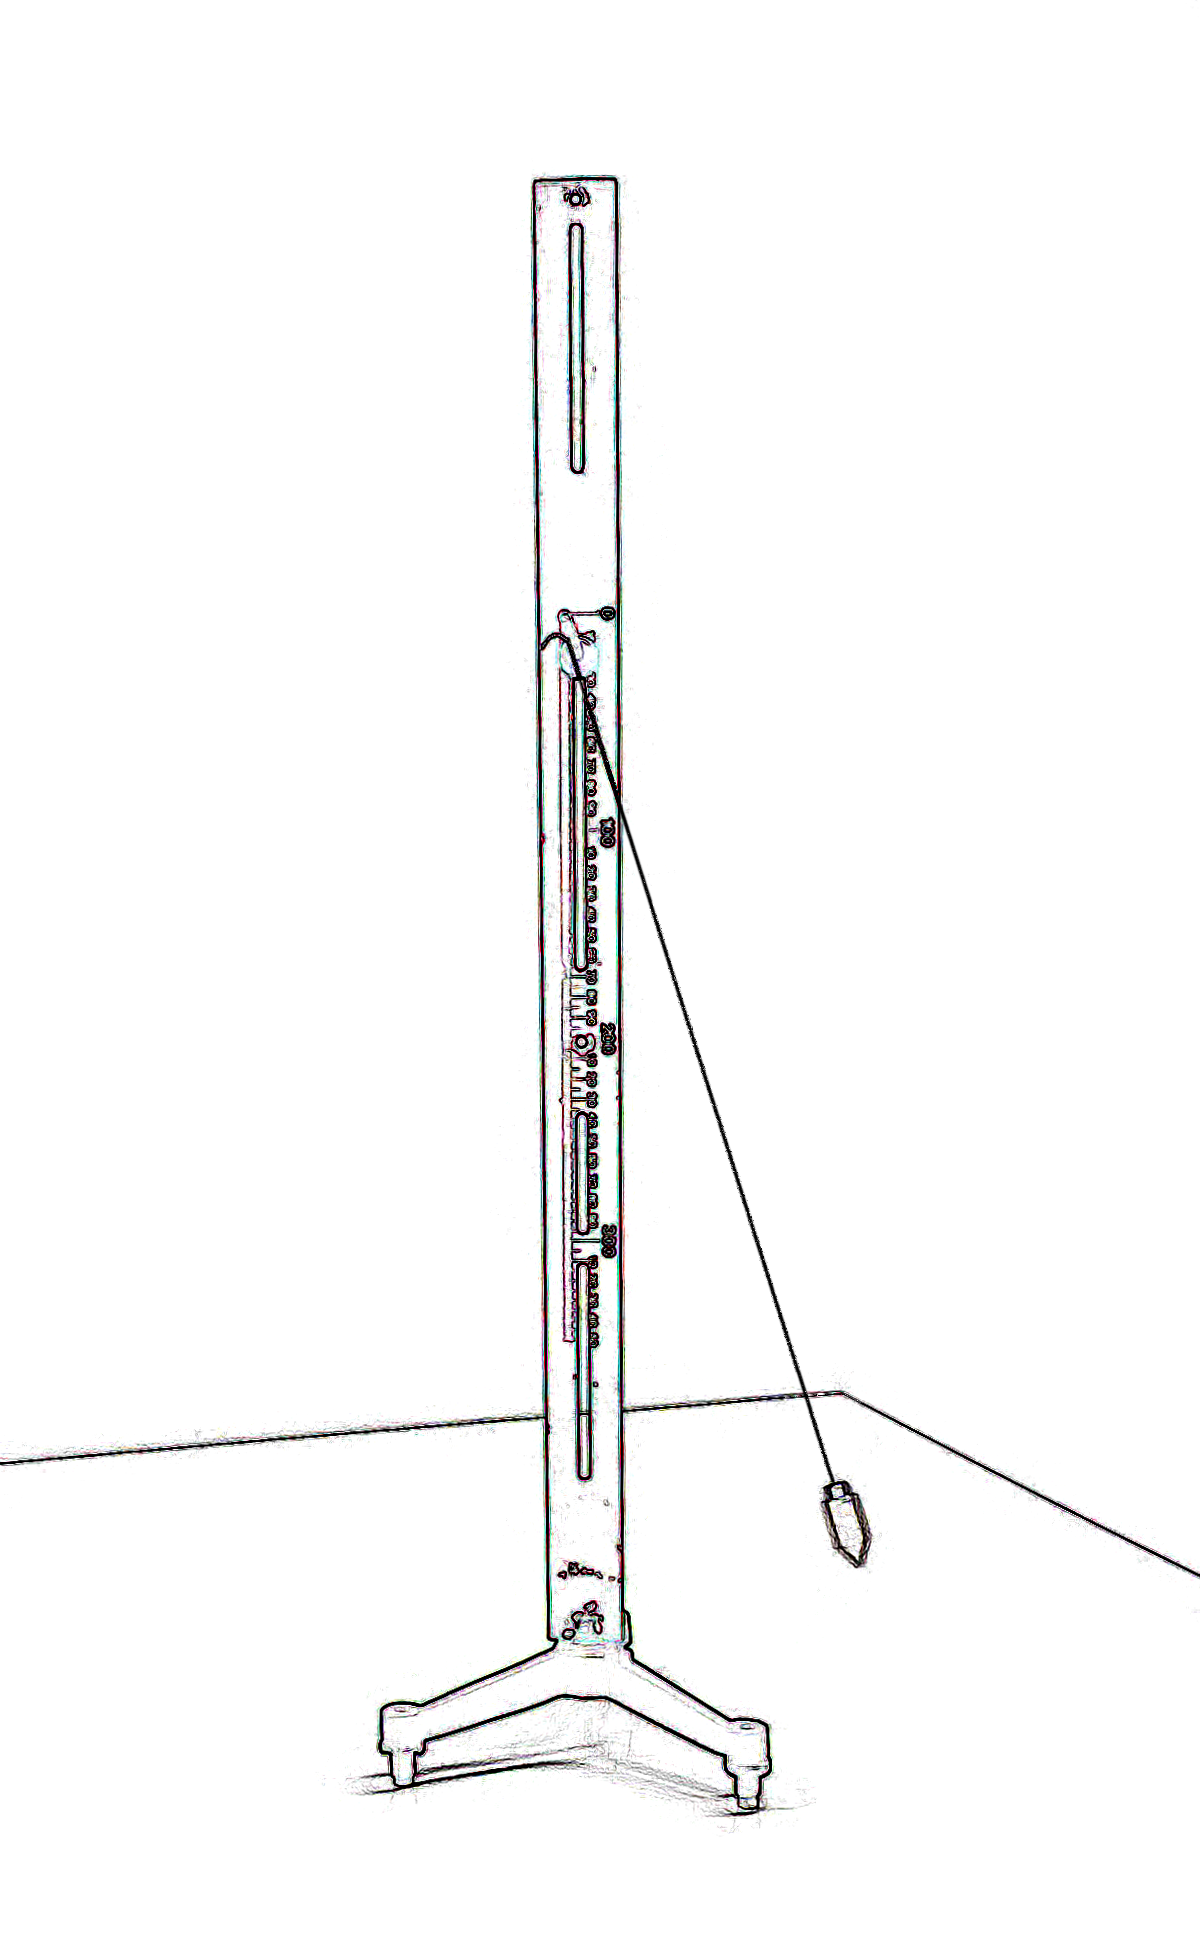
\includegraphics[width=\textwidth]{Ilustrations/Pendulo_simples.png}
	\caption{Pêndulo simples.}
\end{marginfigure}
%
onde o sinal está relacionado ao fato de que a força tem sempre direção contrária ao deslocamento. A aceleração $a$ se refere à derivada segunda da posição ao longo do arco $s$ descrito pelo objeto, portanto podemos escrever
\begin{equation}
	\frac{d^2s}{dt^2} + g\sin\theta = 0.
\end{equation}
%
\begin{marginfigure}[1cm]
\centering
\begin{tikzpicture}[>=Stealth]
	\shade[top color=white,bottom color=gray] (-1,0) rectangle +(2,0.3);
	\draw (-1,0) -- (1,0);
	\draw[dotted] (0,0) -- (0,-1.5);
	\draw (0,-3) arc[start angle = 270, end angle = 300, radius = 3] node[above, midway]{$s$} -- node[right] {$L$} (0,0);
	\draw[dotted] (canvas polar cs:radius=3cm,angle=300) arc[start angle = 300, end angle = 330, radius = 3];
	\draw (0,-0.7) arc[start angle = 270, end angle = 300, radius = 0.7] node[below = 0.05,midway] {$\theta$};
	\draw[fill] (canvas polar cs:radius=3cm,angle=300) circle[radius = 0.1] node[right=2pt] {$m$};
	\draw[->] (canvas polar cs:radius=3cm,angle=300) -- +(canvas polar cs:radius = 0.866025404 cm, angle = 120) node [midway, right]{$\vec{T}$};
	\draw[->] (canvas polar cs:radius=3cm,angle=300) -- node[left]{$\vec{P}$} +(0,-1);
	\draw[dashed,rotate=30] (canvas polar cs:radius=3cm,angle=270) ++(1,0) -- +(-2,0);
	\draw[dashed,rotate=30] (canvas polar cs:radius=3cm,angle=270) -- +(0,-1);
\end{tikzpicture}
\caption{Diagrama de corpo livre do pêndulo simples.}
\label{Fig:Pendulo}
\end{marginfigure}
%
\begin{marginfigure}[1cm]
\centering
\begin{tikzpicture}[>=Stealth,scale=1.5]
	\usetikzlibrary{calc}
	\def\centerarc[#1](#2)(#3:#4:#5)% [draw options] (center) (initial angle:final angle:radius)
	{ \draw[#1] ($(#2)+({#5*cos(#3)},{#5*sin(#3)})$) arc (#3:#4:#5); }
	\draw[fill] (0,0) circle[radius = 0.06667];
	\draw[->] (0,0) -- +(canvas polar cs:radius = 0.866025404 cm, angle = 120) node [midway, right]{$\vec{T}$};
	\draw[->] (0,0) -- node[left]{$\vec{P}$} +(0,-1);
	\draw[dashed,rotate=30] (0,0) ++(1,0) -- +(-2,0);
	\draw[dashed,rotate=30] (0,0) -- +(0,-1.2);
	\draw (0,0) +(0,-0.5) arc[start angle = 270, end angle = 300, radius = 0.5] node[below = 0.05,midway] {$\theta$};
	\draw[->,rotate=30] (0,0) -- node[above]{$P_t$} +(-0.5,0);
	\draw[dotted,rotate=30] (-0.5,-0.866025404) -- +(0,0.866025404);
	\draw[->,rotate=30] (0,0) -- node[right]{$P_r$} +(0,-0.866025404);
	\draw[dotted,rotate=30] (-0.5,-0.866025404) -- +(0.5,0);
	\centerarc[dotted](canvas polar cs:radius = 3 cm, angle = 120)(280:320:3);
\end{tikzpicture}
\caption{Decomposição da força peso em uma componente tangencial à trajetória circular e em uma componente ao longo da reta radial que liga o centro da trajetória à posição do corpo.}
\end{marginfigure}
%
Lembrando ainda que $s = L\theta$, podemos reescrever a equação acima como
\begin{equation}
	\frac{d^2\theta}{dt^2} + \frac{g}{L}\sin\theta = 0.
\end{equation}

Até este momento, a equação acima descreve o movimento de um pêndulo para qualquer valor de amplitude e, devido à função seno, não temos uma oscilação harmônica. Uma propriedade do seno, no entanto, é que para valores pequenos de $\theta$, $\sen\theta \approx \theta$. Isso pode ser visto através de uma expansão em série:
\begin{equation}
	\sen\theta = \theta -\frac{\theta^3}{3!}+\frac{\theta^5}{5!}-\frac{\theta^7}{7!}+\dots,
\end{equation}
%
onde $\theta$ é dado em radianos. Se $\theta$ é pequeno (muito menor que 1), $\theta^3$ é menor ainda, portanto os termos de ordem maior que $\theta$ são desprezíveis para pequenas oscilações. Logo
\begin{equation}
	\frac{d^2\theta}{dt^2} + \frac{g}{L}\theta = 0.
\end{equation}
%
Como a equação acima tem a mesma forma que a Equação~\ref{Eq:EquacaoDiferencialOHS}, concluímos que o movimento para o pêndulo simples também é harmônico, sendo que seu período é dado por
\begin{equation}
	T = 2\pi \sqrt{\frac{L}{g}}.
\end{equation}


%%%%%%%%%%%%%%%%%%%%%%%%%%%%%%%%%%%%%%%%%%%%%%%%%%%%%%%%%%%%%%%%%%%%%%%%%%%%%%%
\section{Experimento}
%%%%%%%%%%%%%%%%%%%%%%%%%%%%%%%%%%%%%%%%%%%%%%%%%%%%%%%%%%%%%%%%%%%%%%%%%%%%%%%

%%%%%%%%%%%%%%%%%%%%%%
\subsection{Objetivos}
%%%%%%%%%%%%%%%%%%%%%%

\begin{itemize}
	\item Verificar a relação entre o período e a massa para um sistema massa-mola.
	\item Verificar a relação entre o período e o comprimento de um pêndulo simples.
	\item Determinar a constante elástica de uma mola através do período de oscilação de um sistema massa-mola.
	\item Determinar a aceleração da gravidade através do período de oscilação de um pêndulo simples.
\end{itemize}

%%%%%%%%%%%%%%%%%%%%%%%%%%%%%%%%%%%%%%%%%%%%%%%%%%%%%%%%%%%%%%%%%%%%%%%%%%%%%%%
\section{Material Necessário}
%%%%%%%%%%%%%%%%%%%%%%%%%%%%%%%%%%%%%%%%%%%%%%%%%%%%%%%%%%%%%%%%%%%%%%%%%%%%%%%

\begin{itemize}
	\item Suporte vertical com haste horizontal;
	\item Mola;
	\item Ganchos e anilhas;
	\item Balança;
	\item Cronômetro;
	\item Fio flexível;
	\item Corpo pequeno a que se possa prender um fio;
	\item Régua milimetrada de \np[cm]{100,00}.
	\item Transferidor.
\end{itemize}

%%%%%%%%%%%%%%%%%%%%%%%%%%%%%%%%%%%%%%%%%%%%%%%%%%%%%%%%%%%%%%%%%%%%%%%%%%%%%%%
\section{Procedimento Experimental}
%%%%%%%%%%%%%%%%%%%%%%%%%%%%%%%%%%%%%%%%%%%%%%%%%%%%%%%%%%%%%%%%%%%%%%%%%%%%%%%

%%%%%%%%%%%%%%%%%%%%%%%%%%%%%%%
\subsection{Sistema massa-mola}
%%%%%%%%%%%%%%%%%%%%%%%%%%%%%%%

\begin{enumerate}
\item Prenda uma extremidade da mola à haste horizontal do suporte e a disponha verticalmente.
\item Afira a massa de um gancho com uma anilha, anotando o valor na Tabela~\ref{Tab:DadosMassaMola}. Prenda-os à extremidade inferior da mola.
\item Desloque o gancho e a anilha alguns centímetros para baixo e solte. Deixe o sistema completar 10 oscilações, cronometrando o tempo necessário para efetuá-las. Cuidado para não exceder a amplitude máxima para a compressão da mola. Utilize como erro para o cronômetro\footnote{Em um cronômetro manual, o erro é dominado pelo tempo de reação do operador. Por isso, o valor típico do desvio padrão de uma medida efetuada com um cronômetro deste tipo não coincide com o valor da menor divisão da escala --~se o equipamento for não-analógico~--, ou com a metade dela --~se o equipamento for analógico~--.} o valor de \np[s]{0,2}.
\item Anote os resultados para o tempo necessário para completar as 10 oscilações na Tabela~\ref{Tab:DadosMassaMola}. Utilize unidades do SI.
\item Adicione anilhas ao gancho, uma a uma, e repita o processo acima para cada adição. Anote os valores de massa do gancho com as anilhas e o tempo correspondente de oscilação. Adicione tantas anilhas quanto possível, tomando o cuidado de não danificar a mola.
\end{enumerate}

%%%%%%%%%%%%%%%%%%%%%%%%%%%%
\subsection{Pêndulo simples}
%%%%%%%%%%%%%%%%%%%%%%%%%%%%

\begin{enumerate}
	\item Prenda o corpo pequeno à extremidade de um fio flexível.
	\item Prenda prenda a outra extremidade do fio à haste horizontal do suporte, de forma que a distância entre a haste de sustentação e o centro de massa do corpo seja de aproximadamente \np[cm]{100,00}. Solte o corpo de forma que o fio fique esticado e o corpo se mantenha parado, sustentado pelo fio.
	\item Desloque o corpo lateralmente, de forma que o ângulo entre o fio e a vertical não exceda \np[\tcdegree]{10,0}. Deixe o corpo completar 10 oscilações, cronometrando o tempo necessário. Anote o valor do comprimento do fio e do tempo para as 10 oscilações na Tabela~\ref{Tab:DadosPendulo}. Utilize unidades do SI.
	\item Diminua o tamanho do fio em \np[cm]{5,00} e calcule o novo tempo necessário para completar as 10 oscilações, anotando as informações na Tabela~\ref{Tab:DadosPendulo}.
	\item Repita o processo acima até um comprimento mínimo de \np[cm]{45,00}.
\end{enumerate}


%%%%%%%%%%%%%%%%%%%%%%%%%%%%%%%%%%%%%%%%%%%%%%%%%%%%%%%%%%%%%%%%%%%%%%%%%%%%%%%
%%%%%%%%%%%%%%%%%%%%%%%%%%%%%%%%%%%%%%%%%%%%%%%%%%%%%%%%%%%%%%%%%%%%%%%%%%%%%%%
%%%%%%%%%%%%%%%%%%%%%%%%%%%%%%%%%%%%%%%%%%%%%%%%%%%%%%%%%%%%%%%%%%%%%%%%%%%%%%%
%%%%%%%%%%%%%%%%%%%%%%%%%%%%%%%%%%%%%%%%%%%%%%%%%%%%%%%%%%%%%%%%%%%%%%%%%%%%%%%
\cleardoublepage

\noindent{}{\huge\textit{Oscilações}}

\vspace{15mm}

\begin{fullwidth}
\noindent{}\makebox[0.6\linewidth]{Turma:\enspace\hrulefill}\makebox[0.4\textwidth]{  Data:\enspace\hrulefill}
\vspace{5mm}

\noindent{}\makebox[0.6\linewidth]{Aluno(a):\enspace\hrulefill}\makebox[0.4\textwidth]{  Matrícula:\enspace\hrulefill}

\noindent{}\makebox[0.6\linewidth]{Aluno(a):\enspace\hrulefill}\makebox[0.4\textwidth]{  Matrícula:\enspace\hrulefill}

\noindent{}\makebox[0.6\linewidth]{Aluno(a):\enspace\hrulefill}\makebox[0.4\textwidth]{  Matrícula:\enspace\hrulefill}

\noindent{}\makebox[0.6\linewidth]{Aluno(a):\enspace\hrulefill}\makebox[0.4\textwidth]{  Matrícula:\enspace\hrulefill}

\noindent{}\makebox[0.6\linewidth]{Aluno(a):\enspace\hrulefill}\makebox[0.4\textwidth]{  Matrícula:\enspace\hrulefill}
\end{fullwidth}

\vspace{5mm}

%%%%%%%%%%%%%%%%%%%%%%%%%%%%%%%%%%%%%%%%%%%%%%%%%%%%%%%%%%%%%%%%%%%%%%%%%%%%%%%
\section{Questionário}
%%%%%%%%%%%%%%%%%%%%%%%%%%%%%%%%%%%%%%%%%%%%%%%%%%%%%%%%%%%%%%%%%%%%%%%%%%%%%%%

\begin{question}[type={exam}]{1}
Apresente os resultados de maneira clara e organizada. Mostre os cálculos requisitados de maneira clara e sucinta, evidenciando o raciocínio desenvolvido.
\end{question}

\begin{question}[type={exam}]{0.75}
Liste os equipamentos utilizados descrevendo o tipo do equipamento, sua resolução, e qual é o seu erro de escala.
\end{question}

\begin{question}[type={exam}]{0.75}
Preencha as tabelas com o número adequado de algarismos significativos, unidades, e erros de escala apropriados. 
\end{question}

\begin{question}[type={exam}]{1.5}
Elabore um gráfico de $T^2 \times m$ para os dados da Tabela~\ref{Tab:DadosMassaMola}. Calcule a reta que melhor representa os dados experimentais utilizando o método dos mínimos quadrados. Mostre a relação entre o coeficiente angular $B$ e a constante da mola $k$, e calcule o valor desta última. \emph{Utilize as unidades do SI para efetuar a regressão linear para obter resultados de mais fácil interpretação.}
\end{question}
 
\begin{question}[type={exam}]{1.5}
Elabore um gráfico de $T^2 \times L$ para os dados da Tabela~\ref{Tab:DadosPendulo}. Calcule a reta que melhor representa os dados experimentais utilizando o método dos mínimos quadrados. Mostre a relação entre o coeficiente angular $B$ e a aceleração da gravidade $g$, e calcule o valor desta última. \emph{Utilize as unidades do SI para efetuar a regressão linear para obter resultados de mais fácil interpretação.}
\end{question}

\begin{question}[type={exam}]{1.5}
Calcule o erro associado ao coeficiente angular para a regressão linear dos dados de $T^2 \times m$. Com esse valor e o do próprio coeficiente, calcule o erro associado à constante da mola $k$.
\end{question}

\begin{question}[type={exam}]{1.5}
Calcule o erro associado ao coeficiente angular para a regressão linear dos dados de $T^2 \times L$. Com esse valor e o do próprio coeficiente, calcule o erro associado à constante da mola $g$.
\end{question}

\begin{question}[type={exam}]{1.5}
Através dos resultados obtidos nas questões anteriores, discuta quais objetivos foram atingidos com sucesso, justificando suas conclusões. Se algum objetivo não foi atingido, discuta quais são os possíveis motivos do fracasso e que providências podem ser tomadas para que eles sejam alcançados.
\end{question}

%%%%%%%%%%%%%%%%%%%%%%%%%%%%%%%%%%%%%%%%%%%%%%%%%%%%%%%%%%%%%%%%%%%%%%%%%%%%%%%
\section{Tabelas}
%%%%%%%%%%%%%%%%%%%%%%%%%%%%%%%%%%%%%%%%%%%%%%%%%%%%%%%%%%%%%%%%%%%%%%%%%%%%%%%
\begin{table*}[!htb]
\caption{Dados para a oscilação de um sistema massa-mola e de um pêndulo simples.}
\label{Tab:DadosMassaMola}
	\begin{center}
		\begin{tabular}{p{25mm}p{25mm}p{25mm}p{25mm}}
		\toprule
		$m$ & $T_{10}$ & $T$ & $T^2$ \\
		\midrule
		\cellcolor[gray]{0.89} & \cellcolor[gray]{0.92} & \cellcolor[gray]{0.89} & \cellcolor[gray]{0.92} \\
		\cellcolor[gray]{0.95} & \cellcolor[gray]{0.97} & \cellcolor[gray]{0.95} & \cellcolor[gray]{0.97} \\
		\cellcolor[gray]{0.89} & \cellcolor[gray]{0.92} & \cellcolor[gray]{0.89} & \cellcolor[gray]{0.92} \\
		\cellcolor[gray]{0.95} & \cellcolor[gray]{0.97} & \cellcolor[gray]{0.95} & \cellcolor[gray]{0.97} \\
		\cellcolor[gray]{0.89} & \cellcolor[gray]{0.92} & \cellcolor[gray]{0.89} & \cellcolor[gray]{0.92} \\
		\cellcolor[gray]{0.95} & \cellcolor[gray]{0.97} & \cellcolor[gray]{0.95} & \cellcolor[gray]{0.97} \\
		\bottomrule
		\end{tabular}
	\end{center}
\end{table*}
%
%
\begin{table*}[!htb]
	\caption{Dados para a oscilação de um pêndulo.}
	\label{Tab:DadosPendulo}
	\begin{center}
		\begin{tabular}{p{25mm}p{25mm}p{25mm}p{25mm}}
		\toprule
		  $L$ & $T_{10}$ & $T$ & $T^2$\\
		\midrule
		\cellcolor[gray]{0.89} & \cellcolor[gray]{0.92} & \cellcolor[gray]{0.89} & \cellcolor[gray]{0.92} \\
		\cellcolor[gray]{0.95} & \cellcolor[gray]{0.97} & \cellcolor[gray]{0.95} & \cellcolor[gray]{0.97} \\
		\cellcolor[gray]{0.89} & \cellcolor[gray]{0.92} & \cellcolor[gray]{0.89} & \cellcolor[gray]{0.92} \\
		\cellcolor[gray]{0.95} & \cellcolor[gray]{0.97} & \cellcolor[gray]{0.95} & \cellcolor[gray]{0.97} \\
		\cellcolor[gray]{0.89} & \cellcolor[gray]{0.92} & \cellcolor[gray]{0.89} & \cellcolor[gray]{0.92} \\
		\cellcolor[gray]{0.95} & \cellcolor[gray]{0.97} & \cellcolor[gray]{0.95} & \cellcolor[gray]{0.97} \\
		\cellcolor[gray]{0.89} & \cellcolor[gray]{0.92} & \cellcolor[gray]{0.89} & \cellcolor[gray]{0.92} \\
		\cellcolor[gray]{0.95} & \cellcolor[gray]{0.97} & \cellcolor[gray]{0.95} & \cellcolor[gray]{0.97} \\
		\cellcolor[gray]{0.89} & \cellcolor[gray]{0.92} & \cellcolor[gray]{0.89} & \cellcolor[gray]{0.92} \\
		\cellcolor[gray]{0.95} & \cellcolor[gray]{0.97} & \cellcolor[gray]{0.95} & \cellcolor[gray]{0.97} \\
		\cellcolor[gray]{0.89} & \cellcolor[gray]{0.92} & \cellcolor[gray]{0.89} & \cellcolor[gray]{0.92} \\
		\cellcolor[gray]{0.95} & \cellcolor[gray]{0.97} & \cellcolor[gray]{0.95} & \cellcolor[gray]{0.97} \\
		\bottomrule
		\end{tabular}
	\end{center}
\end{table*}
